%----------------------------------------------------------------------------
%bb defines the bounding box for the pdf
%viewport defines the area of the pdf used
%in sidewaysfigure the last entry in bb moves the caption toward/away the pic
%in sidewaysfigure the second entry in bb moves the pic toward/away the caption
%----------------------------------------------------------------------------
\begin{figure}
\scalebox{0.8}[0.8]{
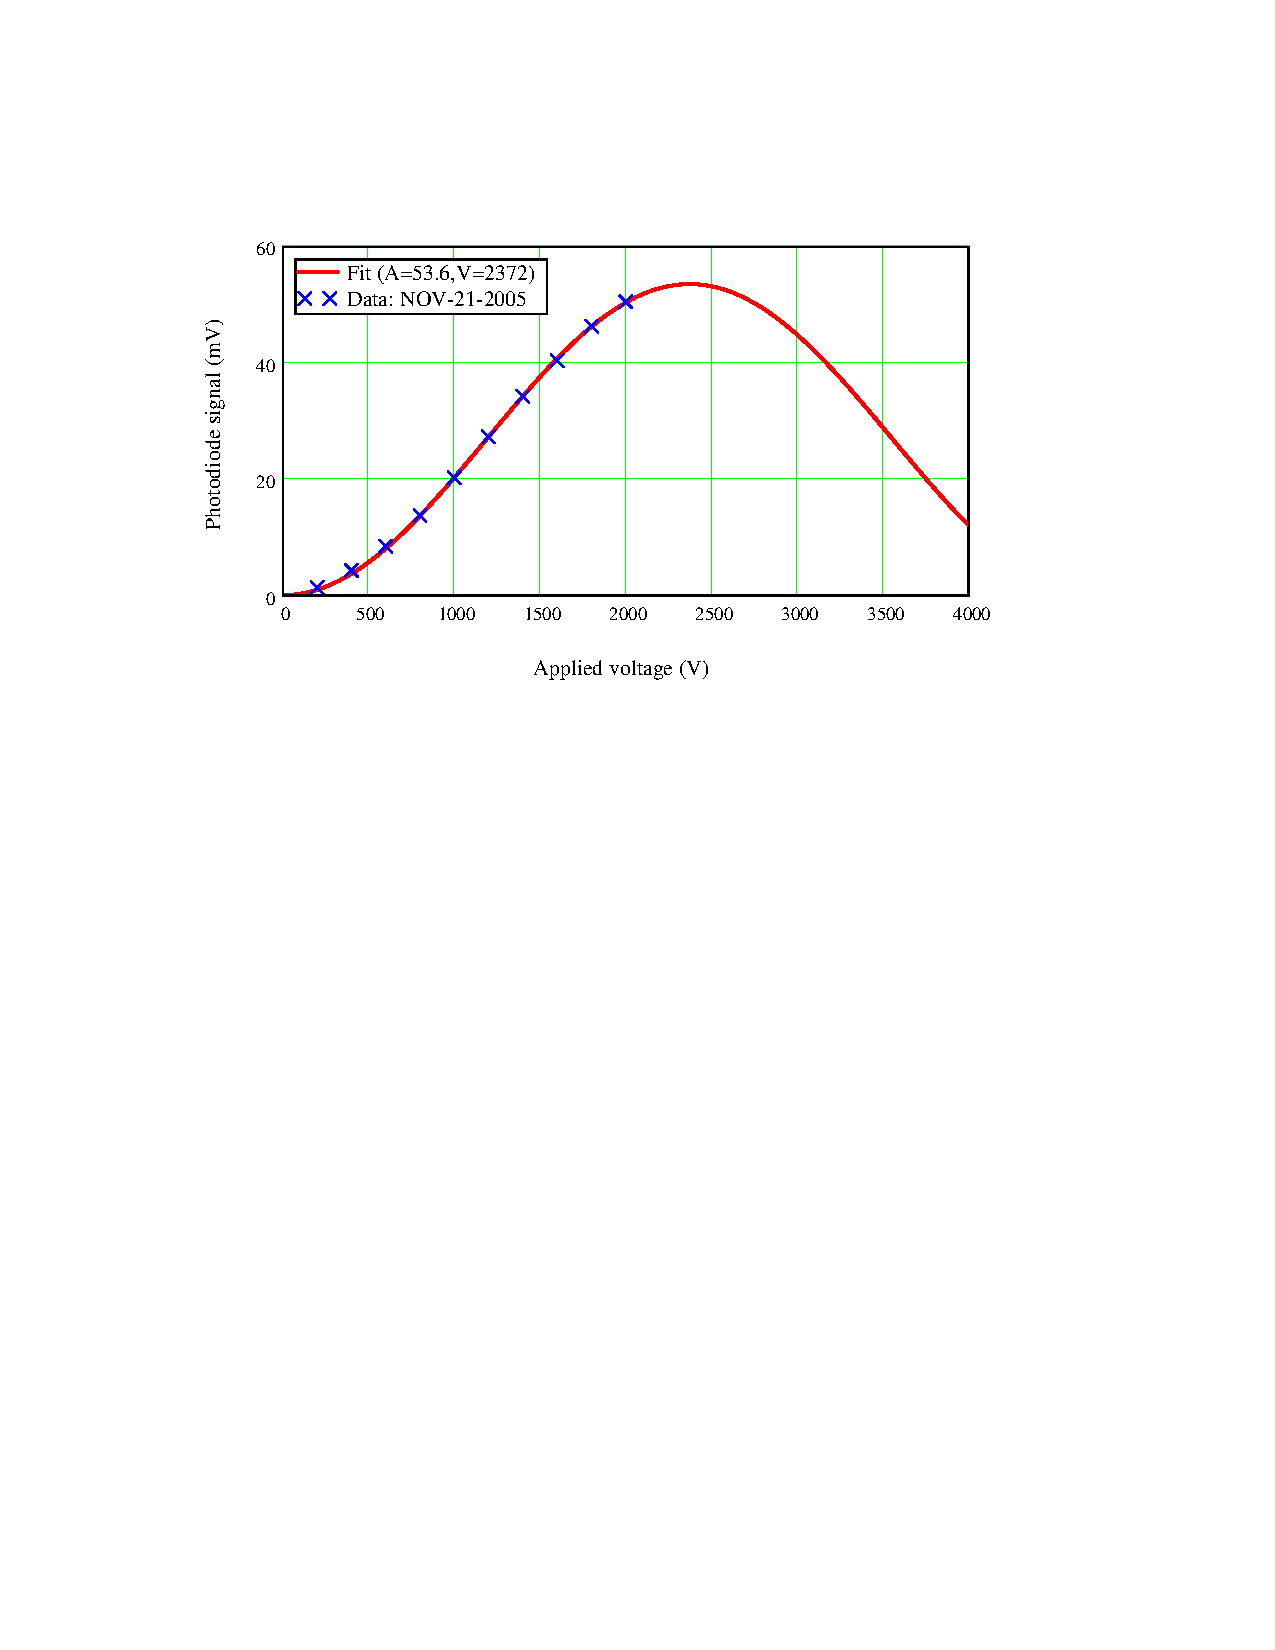
\includegraphics[bb=30 460 481 706]
{fit_532/fit_532.pdf}
}
\caption[DC test of 532nm coated Pockels cell]{DC test of 532nm coated Pockels cell. Since the photodiode signal is 76 mV with the crossed polarizers and Pockels cell removed, the fit value for A (53.6 mV) implies an efficiency of $e \sim 70\%$. Some of the attenuation may be due to the fact the laser wavelength of 543nm is different than the AR coating wavelength. The polarizers will also contribute to the attenuation factor for the system.}
\label{fit_532}
\end{figure}
%----------------------------------------------------------------------------
